\begin{figure}[htp]
\centering
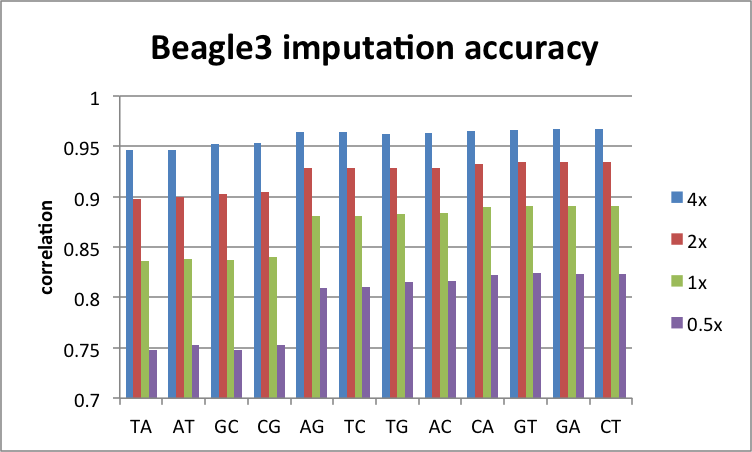
\includegraphics{fig/imp_accu_allele}
\caption[Imputation accuracy for each of the 12 types of biallelic SNPs.]{Imputation accuracy for each of the 12 types of biallelic SNPs. We used the Baganda 4x sequence data and SNP array data to calculate the genotype correlation for each heterozygous allele type. We found that the "mirror" alleles AT/TA and CG/GC for which it can be difficult to determine the relative strand have lower genotype correlations. This is an indication that AT, TA, CG and GC \glspl{SNP} should be avoided in the design of a novel SNP array.}
\label{fig:imp_accu_allele}
\end{figure}